\documentclass{beamer}

\usepackage{natbib}
\bibliographystyle{plain}


\mode<presentation> {

\usetheme{Madrid}

%\setbeamertemplate{footline} % To remove the footer line in all slides uncomment this line
%\setbeamertemplate{footline}[page number] % To replace the footer line in all slides with a simple slide count uncomment this line

%\setbeamertemplate{navigation symbols}{} % To remove the navigation symbols from the bottom of all slides uncomment this line
}

\usepackage{graphicx} % Allows including images
\usepackage{booktabs} % Allows the use of \toprule, \midrule and \bottomrule in tables
\usepackage{tikz}
\usetikzlibrary{bayesnet}

%----------------------------------------------------------------------------------------
%	TITLE PAGE
%----------------------------------------------------------------------------------------

\title[Semantic Frame Induction]{Semantic Frame Induction} % The short title appears at the bottom of every slide, the full title is only on the title page

\author{Eli Drumm, Bill Noble, Jacob Verdegaal} % Your name
\institute[UvA] % Your institution as it will appear on the bottom of every slide, may be shorthand to save space
{
University of Amsterdam \\ % Your institution for the title page
\medskip

}
\date{12/16/14}

\begin{document}

\begin{frame}
\titlepage 
\end{frame}

\begin{frame}
\frametitle{Overview} 
\tableofcontents 
\end{frame}

%----------------------------------------------------------------------------------------
%	PRESENTATION SLIDES
%----------------------------------------------------------------------------------------

%------------------------------------------------
\section{Semantic frames}
%------------------------------------------------


\begin{frame}
  \frametitle{Semantic frames}
  An example\\
  \vspace{10pt}
\begin{tabular}{|l|}
  \hline
  \textit{\small predicate:\normalsize}~~~Transaction\\
  \hline
  \hline
  \textit{\small role 1:\normalsize}~~~ baker\\
  \textit{\small role 2:\normalsize}~~~ Alice\\
  \textit{\small role 3:\normalsize}~~~ bread\\
  \hline
\end{tabular}\\
\vfill
\begin{itemize}
\item Alice buys a bread from the baker
\item The baker sells Alice a bread
  \end{itemize}
\end{frame}

\section{Models}
\begin{frame}
  \frametitle{Model 0 - EM }
  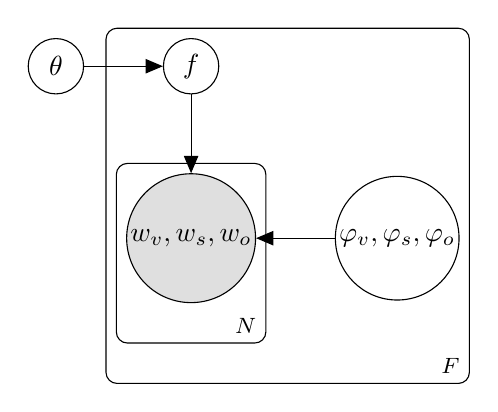
\begin{tikzpicture}
    % Nodes
    \node[obs] (datapoint) {$w_v,w_s,w_o$} ; %
    \node[latent, above=of datapoint] (F) {$f$} ; %
    \node[latent, left=of F] (theta) {$\theta$}; %
    \node[latent, right=of datapoint] (phi) {$\varphi_v,\varphi_s,\varphi_o$}; %
    \edge {theta} {F} ; %
    \edge {F} {datapoint}
    \edge {phi} {datapoint} ; %
    \plate {tuples} { (datapoint) } {$N$}; %
    \plate {} { (tuples) (F) (phi)} {$F$} ; %
  \end{tikzpicture}
\begin{tabbing}
  $N$ \hspace{64pt}\= number of data points\\
  $F$\> number of frames\\
  $\theta$\> distribution over frames\\
  $\varphi_a$ \> distribution per argument $a$ (for frame $f$)\\
  $w_v,w_s,w_o$\> datapoint (verb, subject, object)\\
\end{tabbing}
\end{frame}

\section{Model 1}
\begin{frame}
\frametitle{Model 1 - Gibbs Sampling}
\begin{figure}
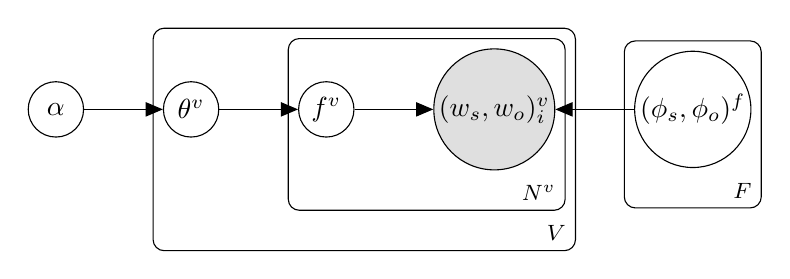
\begin{tikzpicture}[]
    \node[obs]                   (w)     {$(w_s,w_o)^v_i$}; %
    \node[latent, left=of w]     (f)     {$f^v$};
    \node[latent, left=of f]     (theta) {$\theta^v$};
    \node[latent, left=of theta] (alpha) {$\alpha$};
    \node[latent, right=of w]    (phi)   {$(\phi_s,\phi_o)^f$};
    \edge {alpha} {theta};
    \edge {theta} {f};
    \edge {f} {w};
    \edge {phi} {w};
    \plate {frames} {(phi)} {$F$};
    \plate {datapoints} {(f) (w)} {$N^v$};
    \plate {verbs} {(f) (w) (datapoints) (theta)} {$V$};
\end{tikzpicture}
\end{figure}
\end{frame}

\section{Results}
\begin{frame}
  \frametitle{Evaluation metrics}
  \begin{itemize}
  \item Frame coherency: for a datapoint $(v,s,o)$ and a tuple $(v^r,s,o)$ where $v^r$ is a random choses verb: $P(v\mid s,o) \geq P(v^r\mid s,o)$  
  \item Frame correctness: for the top 25 most probable verbs per frame $TV$ and framenet classes of verbs $FN$: \[\frac{2|TV\cap FN|}{|TV|+|FN|}\]
  \end{itemize}
\end{frame}

\begin{frame}
  \frametitle{Results EM - model 0}
\end{frame}

\begin{frame}
  \frametitle{Results Gibbs sampling - model 1}
\end{frame}

\section{References}
\begin{frame}[t,allowframebreaks]
\nocite{*}
\bibliography{refs.bib}
\end{frame}




\end{document}
